\documentclass[../main.tex]{subfiles}

\begin{document}
Il modello descritto in precedenza \'e stato implementato tramite un software scritto in C++.
\section{Classi}
Sfruttando la programmazione a oggetti su cui \'e basato il linguaggio C++ si \'e diviso il modello in varie classi.
\subsection{VehicleType}
La classe a livello inferiore \'e \emph{VehicleType} che, come suggerisce il nome, definisce una tipologia di veicolo.
In questo modello ogni veicolo \'e caratterizzato dai parametri di input nodo sorgente e nodo destinazione.
Tuttavia, per muoversi sul network, ogni tipologia di veicolo necessita anche di una matrice di transizione contenente le probabilità di effettuare o meno un passo in una specifica dimensione.
Questa matrice viene solo dichiarata come parametro della classe e viene impostata dopo la definizione del network.
\subsection{Vehicle}
Dopo aver definito le tipologie di veicoli \'e necessario definire anche i veicoli stessi.
La classe \emph{Vehicle} rappresenta gli agenti che andranno a muoversi sul network stradale.
Un vettore statico di \emph{VehicleType} permette ad ogni veicolo di avere una tipologia definita, tramite un parametro indiciale che determina la posizione nel vettore.
Ogni agente ha inoltre due coordinate che ne definiscono la posizione: nodo attuale e strada attuale.
Per permetterne il movimento nel tempo sono presenti altri due parametri, non necessari in input, rappresentanti la velocità del veicolo, dettata dalla strada sulla quale si trova, e la penalità di tempo che questo deve scontare, dipendente sia dalla velocità del veicolo stesso sia alla densità di veicoli presente sulla strada in cui si trova.
\subsection{Street}
Una volta definiti i veicoli \'e necessario definire le proprietà dei collegamenti tra i vari nodi (incroci) della rete.
Ogni istanza della classe \emph{Street} rappresenta un collegamento tra due nodi.
I parametri da fornire come input per distinguere una strada in maniera univoca sono l'indice del nodo sorgente e l'indice del nodo destinazione.
Si presti ora attenzione al fatto che ogni strada abbia una direzione: considerando due nodi generici $i$ e $j$, la strada che connette $i\to j$ sarà differente dalla strada che connette $j \to i$.
Questa distinzione permette sia una gestione delle densità di veicoli più efficiente e coerente con la realtà, non avendo interferenza tra le corsie, sia l'inserimento di strade a senso unico nella rete.\\
Nella classe \emph{Street} viene poi definito un parametro di controllo del modello, ossia la lunghezza media dei veicoli.
Altri parametri della strada sono la sua lunghezza, il numero $n$ di veicoli su di essa, la velocità massima consentita, il numero di corsie (direzionate come la strada stessa) e la capacità massima $n_{max}$ di veicoli presenti contemporaneamente.
Si noti come mentre un veicolo conosce esattamente la strada in cui si trova ciò non sia vero per la strada in quanto quest'ultima possiede informazione solamente sul numero totale di veicoli presenti su di essa.
La velocità effettiva mantenibile su una strada, essendo un valore altamente dinamico, non viene considerata come parametro (quindi immagazzinato in memoria) ma viene calcolato tramite una funzione quando necessario.
In particolare, l'andamento della velocità su una strada segue la funzione
\begin{equation}
    v(n)=v_{max}\left(1-0.75\frac{n}{n_{max}}\right)
    \label{equation:velocity}
\end{equation}
\begin{figure}[H]
    \centering
    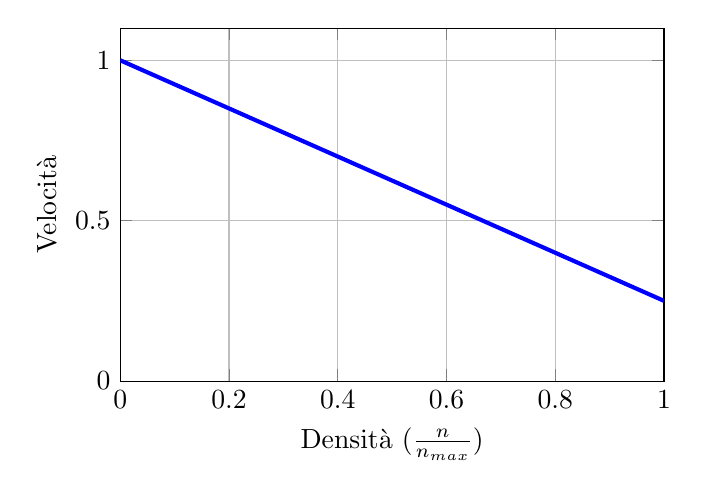
\begin{tikzpicture}
        \begin{axis}[
            grid = both,
            major grid style = {lightgray},
            minor grid style = {lightgray},
            ymin=0,
            xmin=0,
            xmax=1,
            width = 0.7\textwidth,
            height = 0.5\textwidth,
            xlabel = {Densità ($\frac{n}{n_{max}}$)},
            ylabel = {Velocità},]
        \addplot[
            domain = 0:1,
            smooth,
            color = blue,
            line width = 1.5pt,] {1-0.75*x};
        \end{axis}
    \end{tikzpicture}
    \caption[Velocità nel modello]{\emph{Ipotesi dell'andamento della velocità in funzione della densità.}}
    \label{figure:velocity}
\end{figure}
Come visibile in Fig. \ref{figure:velocity} anche una volta raggiunta la densità massima i veicoli non si fermano ma si immettono sulla strada, quando si libera sufficiente spazio, con una velocità minima pari al $25\%$ della velocità massima.
\subsection{Graph}
Ultima classe definita, che comprende tutte le precedenti, \'e la classe \emph{Graph}, la quale costruisce effettivamente il network stradale.
Parametro di input necessario per creare un'istanza \'e la matrice di adiacenza, che definisce le connessioni tra i nodi.
Tramite essa viene poi generato un vettore di puntatori a \emph{Street} che genera le connessioni tra i nodi come strade.\\
Il movimento degli agenti sul network \'e determinato dalla matrice di transizione assegnata alle varie tipologie di veicoli.
Questa viene generata tramite l'utilizzo del famoso algoritmo Dijkstra \cite{dijkstra} e si basa sulla ricerca del \emph{best path}, il percorso a costo (lunghezza) inferiore, dalla posizione dell'agente alla destinazione definita dal suo \emph{VehicleType}.
Si \'e poi deciso di introdurre un parametro di temperatura statistica al network per poter permettere ai veicoli di seguire un percorso differente rispetto al best path fornito dall'algoritmo Dijkstra.
L'algoritmo di evoluzione, infatti, assegna peso 1 ai best path e un peso $\pi$ variabile tra 0 e 1 ai percorsi più lunghi.
Quest'ultimo peso varia in base alla temperatura del sistema secondo la funzione
\begin{equation}
    \pi(T)=\tanh(kT)
\end{equation}
dove $k$ \'e un parametro di controllo del modello.
\begin{figure}[H]
    \centering
    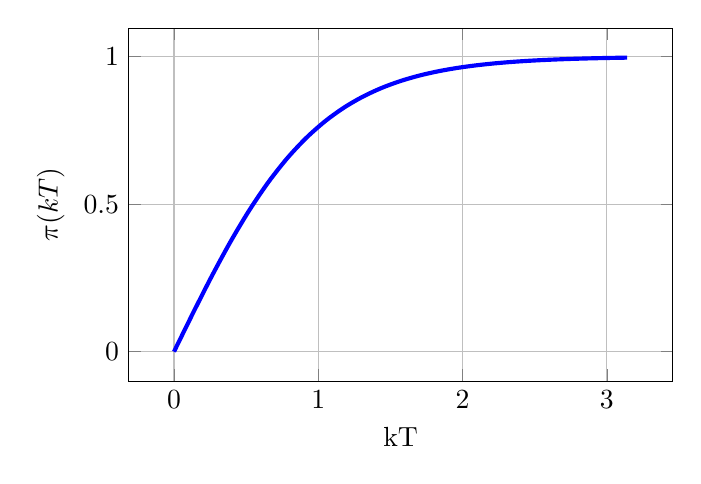
\begin{tikzpicture}
        \begin{axis}[
            grid = both,
            major grid style = {lightgray},
            minor grid style = {lightgray},
            width = 0.7\textwidth,
            height = 0.5\textwidth,
            xlabel = {kT},
            ylabel = {$\pi(kT)$},]
            \addplot[
                domain = 0:3.1415,
                smooth,
                color = blue,
                line width = 1.5pt,] {tanh(x)};
        \end{axis}
    \end{tikzpicture}
    \caption[Temperatura statistica nel modello]{\emph{Probabilità di errore in funzione della temperatura.}}
    \label{figure:temperature}
\end{figure}
Si procede poi alla normalizzazione a 1 di ogni vettore riga della matrice in modo tale da poter ottenere la probabilità di transizione.
Una volta ottenute le probabilità di transizione il sistema può evolvere tenendo presente che:
\begin{itemize}
    \item se un agente prova a muovere su una strada piena questo movimento viene impedito e di fatto si perde uno step temporale;
    \item la velocità di ogni veicolo viene impostata all'ingresso in una strada e non più modificata fino all'ingresso nella strada successiva. 
\end{itemize}

\section{Esecuzione}

\section{Performance}
Il programma \'e stato compilato utilizzando il compilatore gcc-9 su Ubuntu 20.04 nel Windows Subsystem for Linux.
La compilazione \'e stata effettuata utilizzando le flag
\begin{verbatim}
    -O3 -Wall -Wextra -fsanitize=address
\end{verbatim}
in cui:
\begin{itemize}
    \item \emph{O3} indica il livello di ottimizzazione massima volto a ridurre il tempo di esecuzione del programma;
    \item \emph{Wall} e \emph{Wextra} consentono di correggere ogni tipo di warning che sorge in compilazione;
    \item \emph{fsanitize=address} consente di ottenere un'ottima gestione della memoria.
\end{itemize}
\end{document}